\chapter{Results}
\label{cha:results}

%This chapter presents the results. Note that the results are presented
%factually, striving for objectivity as far as possible.  The results
%shall not be analyzed, discussed or evaluated.  This is left for the
%discussion chapter.

%In case the method chapter has been divided into subheadings such as
%pre-study, implementation and evaluation, the result chapter should
%have the same sub-headings. This gives a clear structure and makes the
%chapter easier to write.

%In case results are presented from a process (e.g. an implementation
%process), the main decisions made during the process must be clearly
%presented and justified. Normally, alternative attempts, etc, have
%already been described in the theory chapter, making it possible to
%refer to it as part of the justification.

In this chapter the results are described.
First, the outcome from the exploratory study is presented, followed by the different experiments.
The first experiment, filtering out invalid reports, presents the evaluation of the topic model used to filter out the reports, as well as the specific topics and how they were used in the process.
In the second one, the methods considered and the decisions behind which ones that were appropriate are presented.
Finally, the last section goes through the result of evaluating the different active learning techniques.

\section{Exploratory Study}


\section{Filter Out Invalid Clinical Reports Using Topic Models and Clustering}\label{sec:exp1-result}


Based on these findings, reports were determined to be invalid or not based on if they fulfilled both of the following criteria:
\begin{itemize}
    \item Having either topic 1 or 17 as its most probable topic.
    \item Not having more than 6 prominent topics assigned to it.
\end{itemize}

The evaluation on the validation set can be seen in Table~\ref{tab:exp1-eval}.
In the figure you can also see the results of the logistic regression classifier, which was fitted with the topic vectors as features and the invalid/valid labels as targets.

\begin{table}[h!]
    \centering
    \begin{tabular}{|c|cc|}
        \hline
        & \textbf{Manual Identification} & \textbf{Logistic Regression} \\
        \hline
        \textbf{Precision} & 97.2\% & 98.7\% \\
        \textbf{Recall} & 100\% & 100\% \\
        \textbf{$F_1$-measure} & 98.6\% & 99.4\%\\
        \textbf{Accuracy} & 97.9\% & 99.1\%\\
        \hline
    \end{tabular}
    \caption{The results of the classification of the invalid reports. The manual identification column represents the use of manual interpretation of the LDA topics to find the invalid reports.}
    \label{tab:exp1-eval}
\end{table}

A comparison of how long time it took for the different strategies can be seen in Figure~\ref{fig:al-time-dist}.

\begin{figure}[!ht]
    \centering
    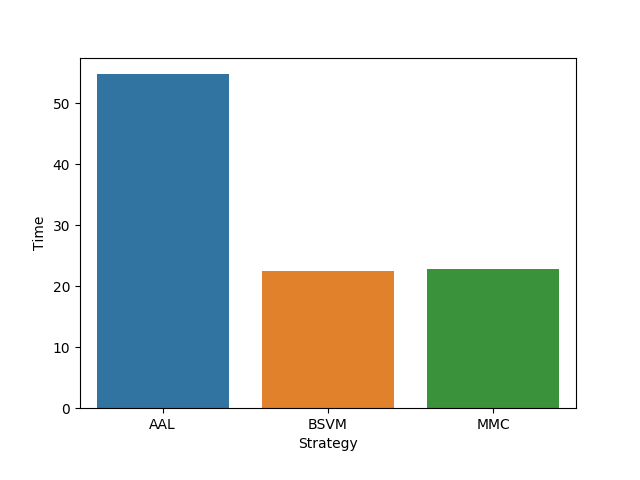
\includegraphics[width=\textwidth]{figures/time-distribution.png}
    \caption{The percentage of time used on the different strategies during one iteration.}
    \label{fig:al-time-dist}
\end{figure}

\section{Alternatives to Labeling at Random}



Based on the knowledge that there exists a pattern, the initial goal was to find some methods that could exploit this.
Some active learning approaches using different forms of clustering, such as Dasgupta et al\@'s approach using hierarchical clustering~\cite{dasgupta2008hierarchical}, would be good contenders.
However, the method described by Dasgupta et al\@. is made for the single-label case with no obvious way of extending the technique into multi-label.
The same applies to the density based technique suggested by Attenberg et al\@.~\cite{attenberg2013class}.

Most of the active learning research seems to be focused on binary, and maybe multi-class classification.
Thus the methods described in Section~\ref{sec:active-learning} where the ones decided on.
Methods that are fully reliant on a models certainty, such as Binary Version Space Minimization (BSVM)~\cite{brinker2006active} are used.
Furthermore, methods incorporating some information about the data in the form of label cardinality is included as well.
These techniques are Maximum Loss Reduction with Maximum Confidence (MMC) and Adaptive Active Learning (AAL)~\cite{yang2009effective, li2013active}.
An attempt to take advantage of the structure of the data is done by selecting the initial samples from different clusters, as described in Section~\ref{sec:exp2-method}.

The plot for evaluating accuracy on the strategies with initial sample sizes of 25, 50 and 100 can be seen in Figure~\ref{fig:al-accuracy-25}, Figure~\ref{fig:al-accuracy-50}, and Figure~\ref{fig:al-accuracy-100} respectively.
Note that when retrieving the initial sample from the clusters, only samples with label cardinality 1 was retrieved after 10 tries.
MMC requires at least two different label cardinalities in the initial sample in order for the logistic regression model to work.
For that reason, MMC with cluster initialization was not evaluated.
In Table~\ref{tab:active-learning-accuracy-25} to Table~\ref{tab:active-learning-accuracy-100} it can be seen how many labels were required to reach a certain accuracy.

\includeaccuracyplot{25}
\includeaccuracyplot{50}
\includeaccuracyplot{100}

\begin{table}
    \centering
    \begin{tabular}{|cccccccc|}
        \hline
        \textbf{Strategy} & \textbf{Initial Sample} & \textbf{75 \%} & \textbf{80 \%} & \textbf{85 \%} & \textbf{87 \%} & \textbf{88 \%} & \textbf{89 \%}\\
        \hline
        BSVM & Random & 475 & 650 & 1100 & 1450 & 1675 & 2425\\
        BSVM & Cluster & 425 & 650 & 1100 & 1575 & 1700 & 2425\\
        MMC & Random & 600 & 775 & 1050 & 1250 & 1575 & N/A\\
        MMC & Cluster & N/A & N/A & N/A & N/A & N/A & N/A\\
        Adaptive & Random & 400 & 575 & 975 & 2425 & N/A & N/A\\
        Adaptive & Cluster & 375 & 550 & 1025 & 2300 & N/A & N/A\\
        Random & Random & 550 & 900 & 1700 & N/A & N/A & N/A\\
        \hline
    \end{tabular}
    \caption{The number of labeled reports in total that the strategies required to achieve the different accuracy values, with initial sample size 25. Only results for the first 2500 data points that were labeled are considered.}
    \label{tab:active-learning-accuracy-25}
\end{table}

\begin{table}
    \centering
    \begin{tabular}{|cccccccc|}
        \hline
        \textbf{Strategy} & \textbf{Initial Sample} & \textbf{75 \%} & \textbf{80 \%} & \textbf{85 \%} & \textbf{87 \%} & \textbf{88 \%} & \textbf{89 \%}\\
        \hline
        BSVM & Random & 450 & 625 & 1075 & 1550 & 1750 & N/A\\
        BSVM & Cluster & 450 & 675 & 1125 & 1600 & 1725 & 2450\\
        MMC & Random & 625 & 775 & 1100 & 1325 & 1675 & N/A\\
        MMC & Cluster & N/A & N/A & N/A & N/A & N/A & N/A\\
        AAL & Random & 375 & 575 & 925 & N/A & N/A & N/A\\
        AAL & Cluster & 425 & 575 & 1075 & N/A & N/A & N/A\\
        Random & Random & 550 & 775 & 1575 & N/A & N/A & N/A\\
        \hline
    \end{tabular}
    \caption{The number of labeled reports in total that the strategies required to achieve the different accuracy values, with initial sample size 50. Only results for the first 2500 data points that were labeled are considered.}
    \label{tab:active-learning-accuracy-50}
\end{table}

\begin{table}
    \centering
    \begin{tabular}{|cccccccc|}
        \hline
        \textbf{Strategy} & \textbf{Initial Sample} & \textbf{75 \%} & \textbf{80 \%} & \textbf{85 \%} & \textbf{87 \%} & \textbf{88 \%} & \textbf{89 \%}\\
        \hline
        BSVM & Random & 400 & 600 & 1125 & 1525 & 1775 & N/A\\
        BSVM & Cluster & 450 & 675 & 1125 & 1600 & 1725 & 2450\\
        MMC & Random & 600 & 750 & 1100 & 1325 & 1675 & N/A\\
        MMC & Cluster & N/A & N/A & N/A & N/A & N/A & N/A\\
        AAL & Random & 350 & 525 & 925 & 2450 & N/A & N/A\\
        AAL & Cluster & 450 & 600 & 1025 & N/A & N/A & N/A\\
        Random & Random & 475 & 775 & 1700 & N/A & N/A & N/A\\
        \hline
    \end{tabular}
    \caption{The number of labeled reports in total that the strategies required to achieve the different accuracy values, with initial sample size 100. Only results for the first 2500 data points that were labeled are considered.}
    \label{tab:active-learning-accuracy-100}
\end{table}

The micro and macro $F_1$-score, recall and precision for the initial sample size of 25 can be seen in Figure~\ref{fig:result-25}.
The same evaluation for the initial sample size of 50 and 100 can be seen in Figure~\ref{fig:result-50} and Figure~\ref{fig:result-100}, respectively.

\includeevaluationplot{25}
\includeevaluationplot{50}
\includeevaluationplot{100}

\section{Evaluating the Label Balance}

The last part to evaluate is how the different Active Learning techniques effected the balance of the labels.
For the Reuters dataset, how the overall distribution of the labels is can be seen in Figure~\ref{fig:class-distribution-reuters}.
After random sampling, the distribution can be seen in Figure~\ref{fig:class-distribution-reuters-random}.
For comparison with the techniques it shows the labels both after 500 labels are added, and 2000.
In order to be able to compare it with the other techniques easily, the plot contains the distribution after both 500 and 2000 labels are acquired.
The distribution after sampling with the original BSVM can be seen in Figure~\ref{fig:class-distribution-reuters-binmin}, and with the initial samples taken from clusters in Figure~\ref{fig:class-distribution-reuters-binmin-clusters}.
For MMC the distribution can be seen in Figure~\ref{fig:class-distribution-reuters-mmc}.
The corresponding plots for Adaptive Active Learning can be seen in Figure~\ref{fig:class-distribution-reuters-adaptive} and Figure~\ref{fig:class-distribution-reuters-adaptive-clusters}.

\begin{figure}
    \centering
    \thirdsubfigimg{distribution-RandomSampling-25-500}{The class distribution from random sampling after 500 labels}
    \thirdsubfigimg{distribution-RandomSampling-25-2000}{The class distribution from random sampling after 2000 labels}
    \caption{The distribution of labels after random sampling}
    \label{fig:class-distribution-reuters-random}
\end{figure}

\begin{figure}
    \centering
    \thirdsubfigimg{distribution-BinaryMinimization-25-500}{The class distribution from BSVM after 500 labels}
    \thirdsubfigimg{distribution-BinaryMinimization-25-2000}{The class distribution from BSVM after 2000 labels}
    \caption{The distribution of labels after BSVM}
    \label{fig:class-distribution-reuters-binmin}
\end{figure}


\begin{figure}
    \centering
    \thirdsubfigimg{distribution-ClusterBinaryMinimization-25-500}{The class distribution from BSVM, with the initial sample from clusters, after 500 labels}
    \thirdsubfigimg{distribution-ClusterBinaryMinimization-25-2000}{The class distribution from BSVM, with the initial sample from clusters, after 2000 labels}
    \caption{The distribution of labels after BSVM with clustering}
    \label{fig:class-distribution-reuters-binmin-clusters}
\end{figure}

\begin{figure}
    \centering
    \thirdsubfigimg{distribution-MMC-25-500}{The class distribution from MMC after 500 labels}
    \thirdsubfigimg{distribution-MMC-25-2000}{The class distribution from MMC after 2000 labels}
    \caption{The distribution of labels after MMC}
    \label{fig:class-distribution-reuters-mmc}
\end{figure}

\begin{figure}
    \centering
    \thirdsubfigimg{distribution-AdaptiveLearner-25-500}{The class distribution from Adaptive Active Learning after 500 labels}
    \thirdsubfigimg{distribution-AdaptiveLearner-25-2000}{The class distribution from Adaptive Active Learning after 2000 labels}
    \caption{The distribution of labels after Adaptive Active Learning}
    \label{fig:class-distribution-reuters-adaptive}
\end{figure}

\begin{figure}
    \centering
    \thirdsubfigimg{distribution-ClusterAdaptiveLearner-25-500}{The class distribution from Adaptive Active Learning, with the initial sample from clusters, after 500 labels}
    \thirdsubfigimg{distribution-ClusterAdaptiveLearner-25-2000}{The class distribution from Adaptive Active Learning, with the initial sample from clusters, after 2000 labels}
    \caption{The distribution of labels after Adaptive Active Learning with clustering}
    \label{fig:class-distribution-reuters-adaptive-clusters}
\end{figure}

In Table~\ref{tab:distribution-result-500} the results of the evaluation after 500 new labels can be seen.
The corresponding table for the evaluation after 2000 new labels can be seen in Table~\ref{tab:distribution-result-2000}.

\begin{table}[h!]
    \centering
    \begin{tabular}{|ccccc|}
        \hline
        \textbf{Strategy} & \textbf{Initial Sample} & \textbf{Top Class} & \textbf{Top 3 Classes} & \textbf{Small/Big Ratio}\\
        \hline
        Random & Random &  34.9 \% & 65.5 \% & 32.0 \\
        BSVM & Random &  22.0 \% & 49.8 \% & 45.0 \\
        BSVM & Clusters & 19.8 \% & 49.0 \% & 80.0 \\
        Adaptive & Random & 14.8 \% & 38.5 \% & 5.4 \\
        Adaptive & Clusters & 14.5 \% & 38.2 \% & 6.65 \\
        MMC & Random & 13.1 \% & 35.2 \% & 8.2 \\
        \hline
    \end{tabular}
    \caption{The results after analyzing the label distribution after 500 new labels has been added.}
    \label{tab:distribution-result-500}
\end{table}

\begin{table}[h!]
    \centering
    \begin{tabular}{|ccccc|}
        \hline
        \textbf{Strategy} & \textbf{Initial Sample} & \textbf{Top Class} & \textbf{Top 3 Classes} & \textbf{Small/Big Ratio}\\
        \hline
        Random & Random & 36.65 \% & 64.6 \% & 29.4 \\
        BSVM & Random & 16.0 \% & 42.4 \% & 7.5 \\
        BSVM & Clusters & 15.7 \% & 41.5 \% & 7.3 \\
        Adaptive & Random & 36.4 \% & 56.2 \% & 43.4 \\
        Adaptive & Clusters & 34.5 \% & 54.8 \% & 41.0 \\
        MMC & Random & 16.7 \% & 41.2 \% & 9.3 \\
        \hline
    \end{tabular}
    \caption{The results after analyzing the label distribution after 2000 labels has been added.}
    \label{tab:distribution-result-2000}
\end{table}